\documentclass[12pt, a4paper, oneside]{ctexart}
\usepackage{amsmath, amsthm, amssymb, bm, color, graphicx, geometry, mathrsfs,extarrows, braket, booktabs, array}
\usepackage[colorlinks,linkcolor=red,anchorcolor=blue,citecolor=blue,urlcolor=blue,menucolor=black]{hyperref}
%%%% 设置中文字体 %%%%
\setCJKmainfont{方正新书宋_GBK.ttf}[ BoldFont = 方正小标宋_GBK, ItalicFont = 方正楷体_GBK]
%%%% 设置英文字体 %%%%
\setmainfont{Times New Roman}
\setsansfont{Calibri}
\setmonofont{Consolas}

\linespread{1.4}
%\geometry{left=2.54cm,right=2.54cm,top=3.18cm,bottom=3.18cm}
\geometry{left=1.84cm,right=1.84cm,top=2.18cm,bottom=2.18cm}
\newcounter{problem}  % 问题序号计数器
\newenvironment{problem}{\stepcounter{problem}\par\noindent\textbf{题目\arabic{problem}. }}{\smallskip\par}
\newenvironment{solution}[1][]{\par\noindent\textbf{#1解答. }}{\smallskip\par}
\newenvironment{note}{\par\noindent\textbf{注记. }}{\smallskip\par}

\usepackage{minted}
\renewcommand{\theFancyVerbLine}{
    \sffamily\textcolor[rgb]{0.5,0.5,0.5}{\scriptsize\arabic{FancyVerbLine}}} % 修改代码前序号大小
\newmintinline{python}{linenos, breaklines, frame=lines, python3}  % 使用\pythoninline{代码}
\newmintinline{cpp}{linenos, breaklines, frame=lines}  % 使用\cppinline{代码}
\newminted{python}{linenos, breaklines, frame=lines, python3}  % 使用\begin{pythoncode}代码\end{pythoncode}
\newminted{cpp}{fontsize=\small, linenos, breaklines, frame=lines}  % 使用\begin{pythoncode}代码\end{pythoncode}
\newmintedfile{python}{linenos, breaklines, frame=lines, python3}  % 使用\pythonfile{代码地址}
\newmintedfile{cpp}{linenos, breaklines, frame=lines}  % 使用\cppfile{代码地址}

%%%% 图片相对路径 %%%%
\graphicspath{{figure/}} % 当前目录下的figure文件夹, {../figure/}则是父目录的figure文件夹

\everymath{\displaystyle} % 默认全部行间公式
\DeclareMathOperator*\uplim{\overline{lim}} % 定义上极限 \uplim_{}
\DeclareMathOperator*\lowlim{\underline{lim}} % 定义下极限 \lowlim_{}
\let\leq=\leqslant % 将全部leq变为leqslant
\let\geq=\geqslant % geq同理

%%%% 一些宏定义 %%%%
\def\bd{\boldsymbol}        % 加粗(向量) boldsymbol
\def\disp{\displaystyle}    % 使用行间公式 displaystyle(默认)
\def\tsty{\textstyle}       % 使用行内公式 textstyle
\def\sign{\text{sign}}      % sign function
\def\wtd{\widetilde}        % 宽波浪线 widetilde
\def\R{\mathbb{R}}          % Real number
\def\N{\mathbb{N}}          % Natural number
\def\Z{\mathbb{Z}}          % Integer number
\def\Q{\mathbb{Q}}          % Rational number
\def\C{\mathbb{C}}          % Complex number
\def\d{\mathrm{d}}          % differential operator
\def\e{\mathrm{e}}          % Euler's number
\def\i{\mathrm{i}}          % imaginary number
\def\re{\mathrm{Re}}        % Real part
\def\im{\mathrm{Im}}        % Imaginary part
\def\res{\mathrm{Res}}      % Residue
\def\L{\mathcal{L}}         % Loss function
\def\O{\mathcal{O}}         % 时间复杂度
\def\wdh{\widehat}          % 宽帽子 widehat
\def\ol{\overline}          % 上横线 overline
\def\ul{\underline}         % 下横线 underline
\def\add{\vspace{1ex}}      % 增加行间距
\def\del{\vspace{-3.5ex}}   % 减少行间距

%%%% 定理类环境的定义 %%%%
\newtheorem{theorem}{定理}

%%%% 基本信息 %%%%
\newcommand{\RQ}{\today} % 日期
\newcommand{\km}{算法设计与分析} % 科目
\newcommand{\bj}{强基数学002} % 班级
\newcommand{\xm}{吴天阳} % 姓名
\newcommand{\xh}{2204210460} % 学号

\begin{document}

%\pagestyle{empty}
\pagestyle{plain}
\begin{center}
    \zihao{3}\textbf{计算机实验}
\end{center}\vspace{-0.2cm}
\begin{solution}{[0/1背包问题]}
    设\cppinline{dp[i][j]}表示从前i个物品中,使用容量为j的背包所能获得的最大价值. 则状态状态转移方程如下
    \begin{equation*}
        dp[i][j] = max\{dp[i-1][j-w[i]]+v[i], dp[i-1][j]\}.
    \end{equation*}
    其中$\max$中的第一项$dp[i-1][j-w[i]]+v[i]$表示在剩余容量为$j$的前提下,选择第$i$个物品所获得的最大价值,则可以从前$i-1$个物品容量为$j-w[i]$所能获得的最大价值加上当前物品的价值$v[i]$得到;$\max$的第二项$dp[i-1][j]$表示不选取第$i$件物品,则直接从前$i-1$件物品容量为$j$的最大价值直接转移得到.

    若$dp[i][j]$是从$\max$的第一项转移得到,则选择了当前物品$i$;否则,从$\max$的第二项转移得到,则没有选择物品$i$. 通过记录$dp[i][j]$从谁转移得到的,即可得知最终选取的物品是哪些. 最终输出可逆向枚举得到.

    实现代码如下:
    \cppfile{01背包.cpp}
\end{solution}

% 下面给一些功能的写法
\iffalse
% 图片模板
\centerline{
    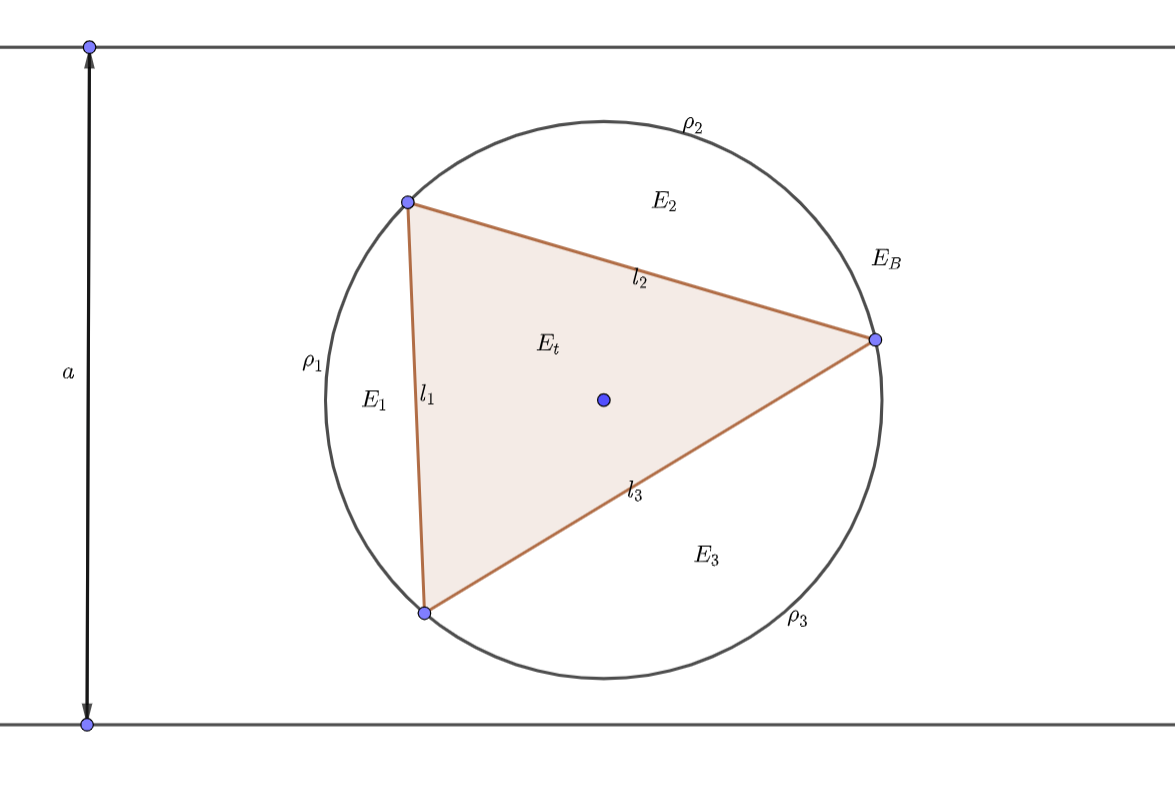
\includegraphics[width=0.8\textwidth]{figure.png}
}
% 表格模板
\renewcommand\arraystretch{0.8} % 设置表格高度为原来的0.8倍
\begin{table}[!htbp] % table标准
    \centering % 表格居中
    \begin{tabular}{p{1cm}<{\centering}p{1cm}<{\centering}p{3cm}<{\centering}p{5cm}<{\centering}} % 设置表格宽度
    %\begin{tabular}{cccc}
        \toprule
        $x_i$ & $f[x_1]$ & $f[x_i,x_{i+1}]$ & $f[x_i,x_{i+1},x_{i+2}]$ \\
        \midrule
        $x_0$ & $f(x_0)$ &                  &                          \\
        $x_0$ & $f(x_0)$ & $f'(x_0)$        &                          \\
        $x_0$ & $f(x_1)$ & $\frac{f(x_1)-f(x_0)}{x_1-x_0}$ & $\frac{f(x_1)-f(x_0)}{(x_1-x_0)^2}-\frac{f'(x_0)}{x_1-x_0}$\\
        \bottomrule
    \end{tabular}
\end{table}

\def\Log{\text{Log}} % 一个简单的宏定义
$\Log$ % 调用方法
\fi

\end{document}